\documentclass[12pt, a4paper]{article}

% --- 基本宏包 ---
\usepackage{geometry}
\usepackage{amsmath}
\usepackage{amssymb}
\usepackage{graphicx}
\usepackage{hyperref}
\usepackage{parskip} % 段落间距
\usepackage{tabularx}
\usepackage{booktabs} % 更美观的表格线

% --- 中文支持 ---
% 使用 xeCJK 宏包,需要使用 XeLaTeX 编译
\usepackage{xeCJK}
%\setCJKmainfont{SimSun} % 设置中文字体,请确保您的系统中有此字体,或替换为您可用的字体,如 FandolSong, STSong, etc.
%\setCJKsansfont{SimHei}
%\setCJKmonofont{FangSong}

% --- 页面与格式设置 ---
\geometry{left=2.5cm, right=2.5cm, top=2.5cm, bottom=2.5cm}
\hypersetup{
    colorlinks=true,
    linkcolor=blue,
    filecolor=magenta,      
    urlcolor=cyan,
    pdftitle={LitaAgentYR Strategy Analysis},
    pdfpagemode=FullScreen,
}
\linespread{1.3} % 行距

% --- 标题 ---
\title{LitaAgentYR 谈判代理策略报告 \\ \large LitaAgentYR Negotiation Agent Strategy Report}
\author{Lita, With assisstance from Gemini}
\date{\today}

\begin{document}
\maketitle
\thispagestyle{empty}
\newpage
\tableofcontents
\newpage

% ==================================================================
% 中文版本
% ==================================================================
\section*{中文报告 (Chinese Report)}

\begin{abstract}
本报告旨在深度剖析 \textbf{LitaAgentYR} 谈判代理的核心策略与算法实现。\textbf{LitaAgentYR} 是一个为供应链管理联盟 (SCML) 竞赛设计的、具有库存感知和动态风险管理能力的代理。报告首先阐述了其基于三层采购与产能约束销售的总体策略,随后详细说明了各个核心方法的功能、变量含义以及它们之间的协同工作流程。最后,报告使用数学公式对代理的接受准则、让步逻辑和对手建模算法进行了精确的形式化表达,并将这些模型与代码实现紧密结合,提供了从理论到实践的全面解析。
\end{abstract}

\section{总体策略}
LitaAgentYR的核心策略是构建一个以\textbf{全局盈利和风险规避}为目标的长期主义代理。它不追求单次谈判的局部最优,而是通过紧密结合库存管理,动态适应市场变化,确保在整个模拟周期内的稳健表现。

\subsection{策略支柱}
\begin{enumerate}
    \item \textbf{库存驱动决策}: 代理的核心大脑是其内部的$InventoryManager$模块。该模块采用“准时制(Just-in-Time)”思想,通过反向传播销售订单来精确规划每日的生产任务,并由此计算出未来每日的原材料精确短缺量。所有谈判行为都以此数据为基础,实现了目标驱动的采购与销售。

    \item \textbf{分层采购逻辑}: 为了平衡成本与风险,代理将采购需求细分为三个不同优先级的层次:
        \begin{itemize}
            \item \textbf{紧急采购 (Emergency)}: 满足当日生产必需的原材料缺口,避免因生产停滞导致违约。在此场景下,代理的接受意愿最高,愿意以接近甚至略高于违约罚金的价格成交。
            \item \textbf{计划采购 (Planned)}: 为满足未来已签订的销售订单而进行的远期采购。此决策的核心是在保证未来销售利润的前提下,权衡采购成本和仓储成本。
            \item \textbf{机会性采购 (Optional)}: 当市场价格远低于历史均价时,在不显著增加库存积压风险的前提下进行战略性囤货,以降低整体原材料成本。
        \end{itemize}

    \item \textbf{产能约束销售}: 代理在对外销售时,严格遵守其每日的生产能力限制。它绝不签订任何在交货日期前无法完成生产的合同,从源头上杜绝了因无法履约而导致的巨额罚款。% TODO:说实话我很怀疑这真的杜绝了吗?代理还是在缴纳penalty,一定在什么地方存在漏洞 此外,inventorypenalty也很高,一定有什么上限没能拦住代理的采购行为

    \item \textbf{动态利润与风险管理}: 代理的利润目标和风险偏好是动态变化的。它会根据游戏阶段、库存健康度、以及历史销售转化率,实时调整其销售的最低利润率$min\_profit\_ratio$和机会性采购的折扣阈值$bargain\_threshold$。

    \item \textbf{帕累托改进的让步策略}: 在还价时,代理不仅仅在价格维度上进行妥协。它会综合评估价格、数量和交货时间,尝试提出对自己更有利,同时又可能被对手接受的多维度组合方案,沿着帕累托前沿探索双赢的可能。
\end{enumerate}

\section{实现与架构}
\subsection{关键组件与变量}
\begin{description}
    \item[LitaAgentYR] 主类,继承自\textbf{$StdSyncAgent$},负责响应SCML环境的各种回调。
    \item[HeuristicSettings] 一个\textbf{$dataclass$},集中存储了代理所有的可调启发式参数,如让步曲线指数、利润率、折扣阈值等,增强了代码的可维护性和可配置性。
    \item[InventoryManager] 库存管理模块,是代理的决策中枢。负责追踪库存批次、管理待处理合同、生成生产计划以及预测物料短缺。
    \item[min\_profit\_ratio] 销售时必须满足的最低利润率。

    \item[bargain\_threshold] 机会性采购的价格折扣阈值。

    \item[partner\_models] 字典,为每个对手存储一个独立的在线逻辑回归模型参数($w_0, w_1$)。
\end{description}

\subsection{核心方法调用流程}
代理的谈判逻辑始于 \textbf{$counter\_all$}方法,这是一个顶层分发器。

\begin{figure}
    \centering
    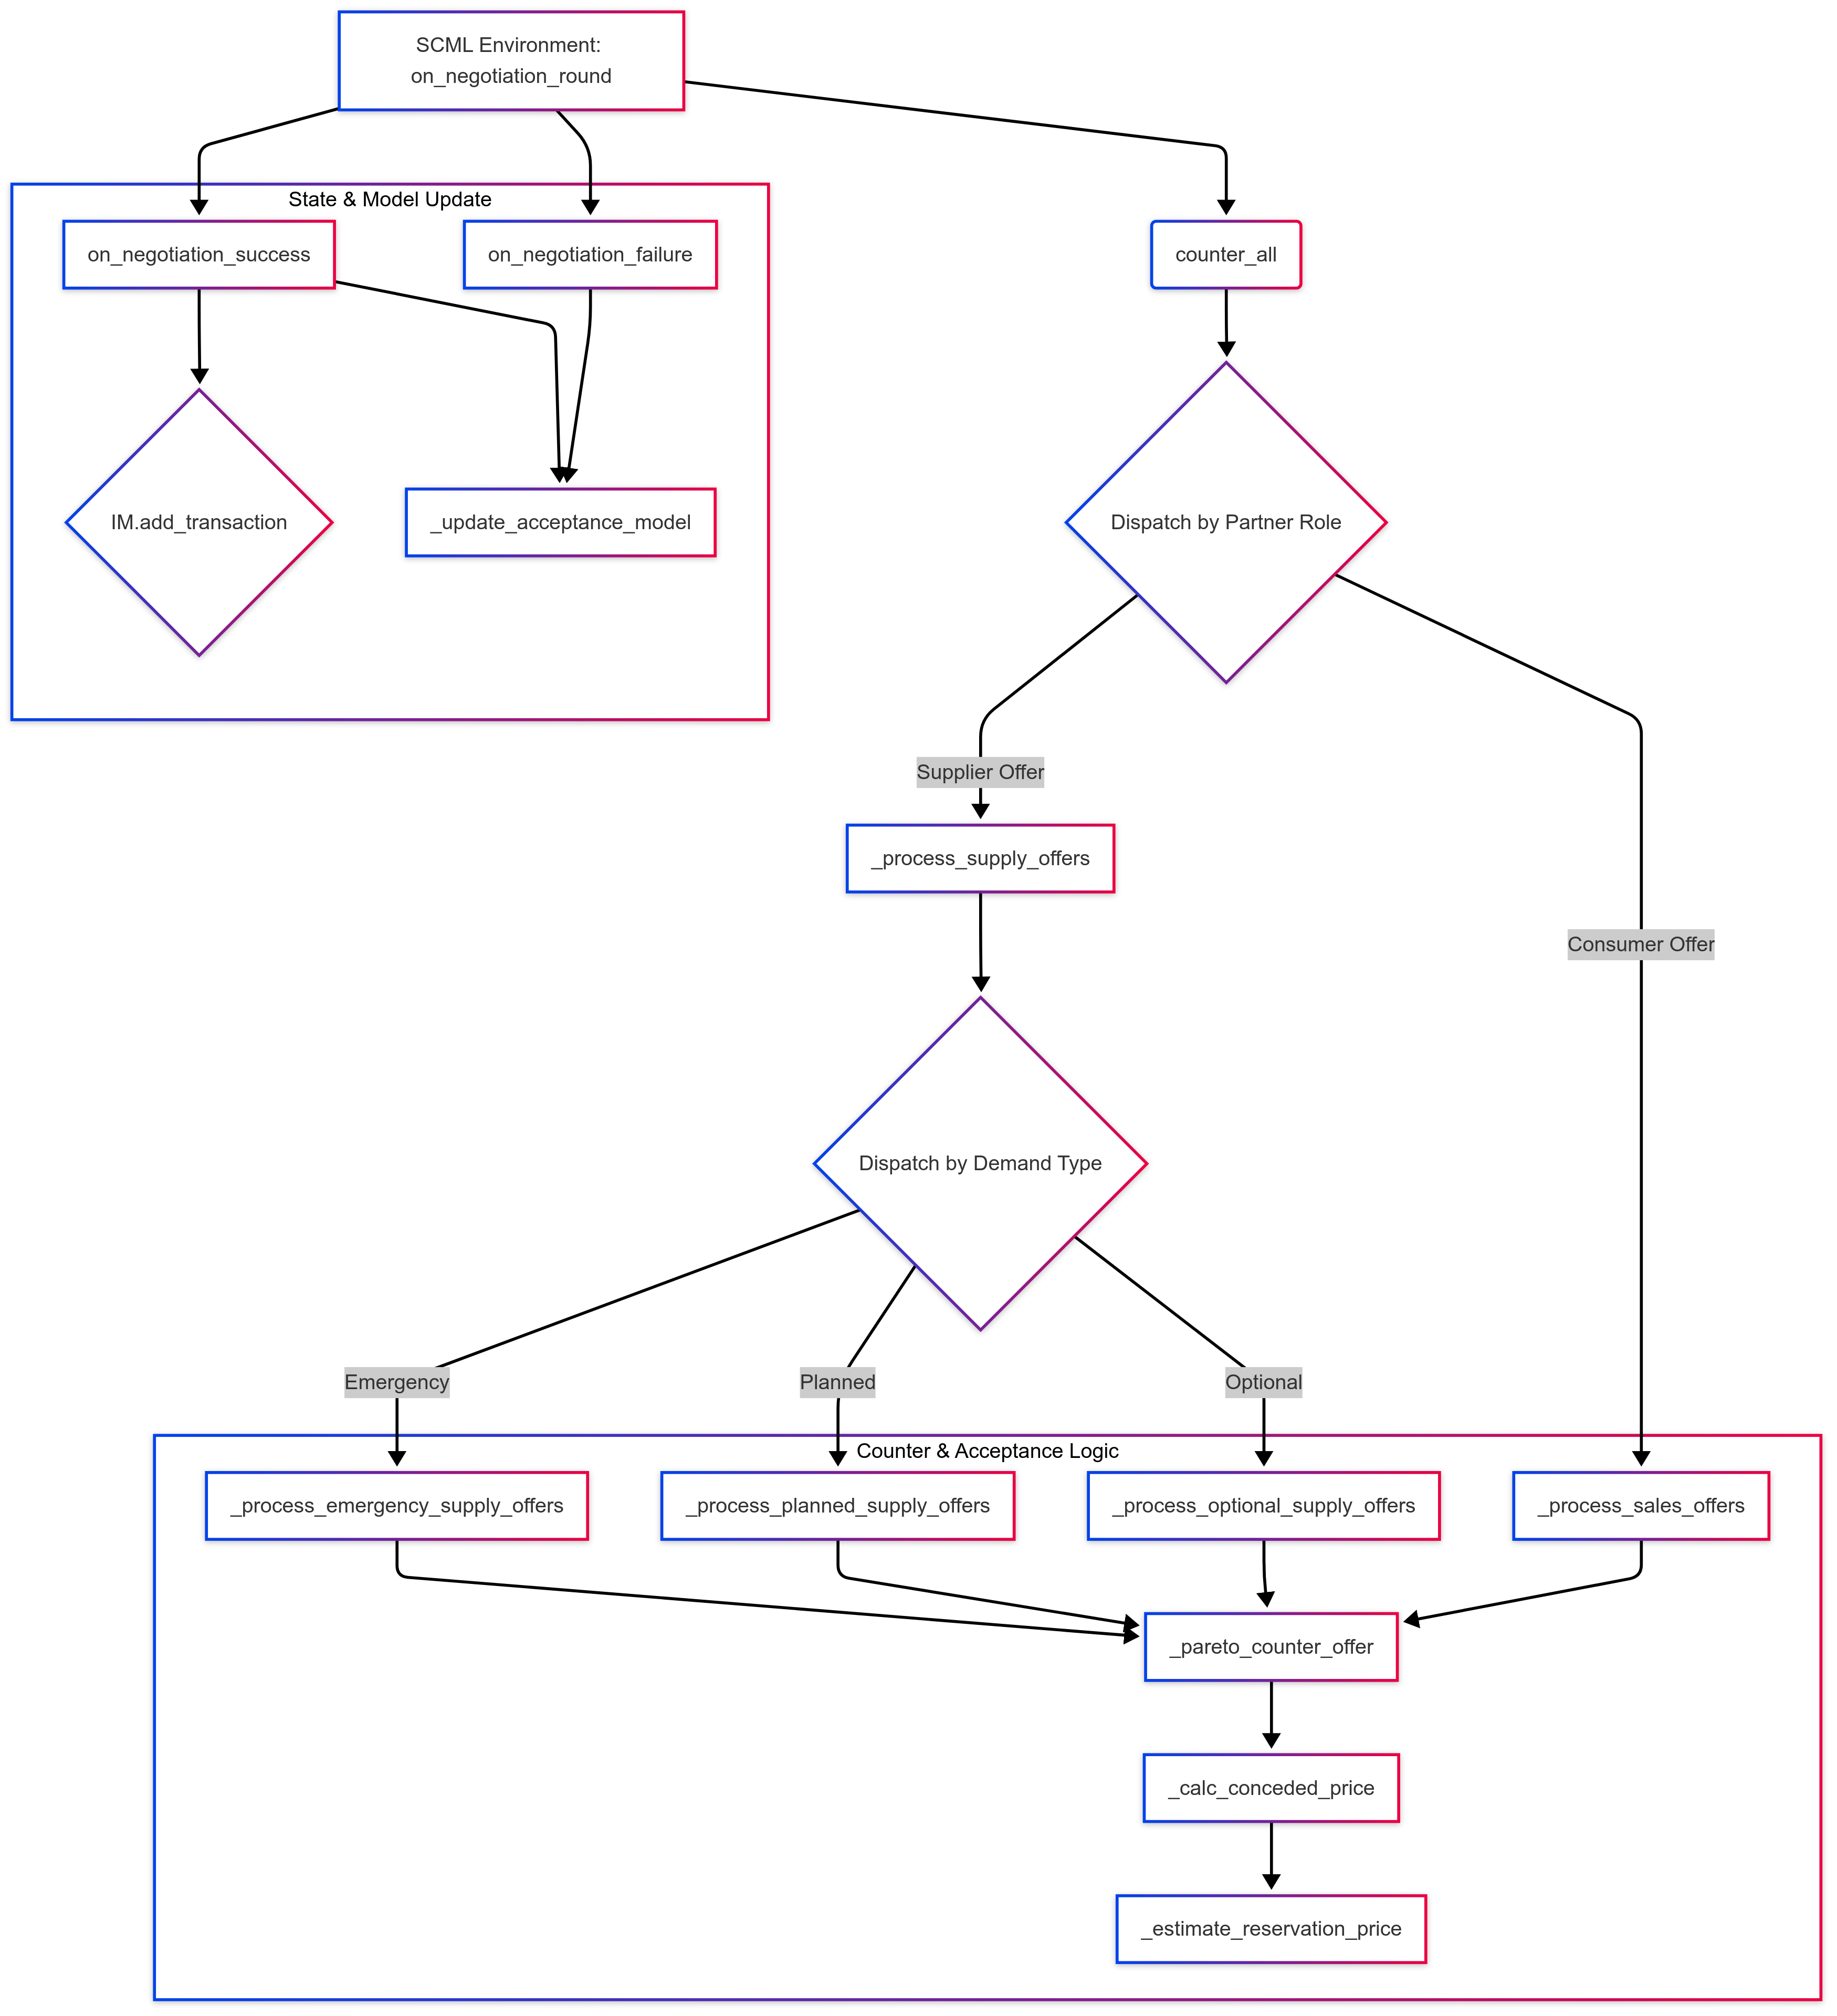
\includegraphics[width=0.75\linewidth]{Editor _ Mermaid Chart-2025-06-08-092514.png}
    \caption{核心方法调用流程}
    \label{fig:enter-label}
\end{figure}
\section{策略的数学建模}

\subsection{接受逻辑 (Acceptance Logic)}
代理的接受决策是情境化的,由四个不同模块的逻辑规则确定。

\begin{enumerate}
\item \textbf{紧急供应}: 接受来自供应商 $i$ 的报价 $(q_i, t_i, p_i)$,如果 $t_i$ 是当天,且满足:
$$
\text{Accept if } (p_i \le \pi) \lor (p_i \le 1.1 \cdot \pi \land t_{\text{rel}} > 0.8)
$$  % Verified by Lita
其中 $\pi$ 是违约罚金 (shortfall\_penalty), $t_{\text{rel}}$ 是相对谈判时间。

\item \textbf{计划性供应}: 接受报价需同时满足盈利性和库存容量限制。
\begin{itemize}
    \item \textbf{盈利性}: $p_{\text{eff}} \le p_{\text{max\_affordable}}$ \\ % Verified by Lita
    其中有效价格 $p_{\text{eff}} = p_i + C_{\text{storage}} \cdot (t_i - t_{\text{today}} - 1)$,包含了仓储成本。可接受的最高采购价 $p_{\text{max\_affordable}}$ 由预估的未来产品售价 $\hat{S}$、加工成本 $C_{\text{proc}}$ 和最低利润率 $m$ 决定:
    $$
    p_{\text{max\_affordable}} = \hat{S} \cdot (1 - m) - C_{\text{proc}}
    $$ % Verified by Lita  这个预期单价代理是首先根据自身观察,然后试着从awi获取,全部失败则换成启发式
    \item \textbf{库存容量}: $q_i \le H(t_i)$, $H(t_i)$ 是在 $t_i$ 时刻的“采购空间”。% Verified by Lita
\end{itemize}

\item \textbf{机会性供应}:  % Verified by Lita
$$
\text{Accept if } p_i \le \bar{p}_{\text{market}} \cdot \delta_{\text{bargain}} \land q_i \le H_{\text{opt}}(t_i)
$$
其中 $\bar{p}_{\text{market}}$ 是市场均价,$\delta_{\text{bargain}}$ 是折扣阈值 (`bargain\_threshold`)。

\item \textbf{销售}:% Verified by Lita
$$
\text{Accept if } q_i \le C_{\text{avail}}(t_i) \land p_i \ge p_{\text{min\_sell}}
$$
其中 $C_{\text{avail}}(t_i)$ 是在 $t_i$ 时刻的可用产能,最低售价 $p_{\text{min\_sell}}$ 由平均原材料成本 $C_{\text{raw\_avg}}$、加工成本 $C_{\text{proc}}$ 和动态利润率 $m_{\text{dynamic}}$ 决定:% Verified by Lita
$$
p_{\text{min\_sell}} = (C_{\text{raw\_avg}} + C_{\text{proc}}) \cdot (1 + m_{\text{dynamic}})
$$
\end{enumerate}

\subsection{让步逻辑 (Concession Logic)}
让步逻辑在 \_calc\_conceded\_price 方法中实现,分三步计算还价 $p^{\text{new}}$。

\begin{enumerate}
\item \textbf{让步乘数 ($\beta$)}:% Verified by Lita
$$
\beta(t_{\text{rel}}, r_{\text{opp}}) = \min\left(1, t_{\text{rel}}^{\gamma} \cdot (1 + r_{\text{opp}})\right)
$$
其中,$t_{\text{rel}}$ 是相对谈判时间,$r_{\text{opp}}$ 是对手的相对让步率,$\gamma$ 是让步曲线的幂 (concession\_curve\_power)。

\item \textbf{目标价格混合 ($p^{\star}$)}: % Verified by Lita 这里的Popp是对手模型计算的 Ptarget是这一轮代理的目标价格,销售时是确保盈利的最低价,紧急采购时是penalty,计划采购时是满足利润的价格,可选采购时是低价阈值价格
$$
p^{\star} = \frac{p_{\text{agent\_target}} + \hat{p}_{\text{opp}}}{2}
$$
其中 $p_{\text{agent\_target}}$ 是代理本轮的理想价格,$\hat{p}_{\text{opp}}$ 是通过对手模型估算的对手保留价格。

\item \textbf{最终价格计算 ($p^{\text{new}}$)}: % Verified by Lita 相当于是一个让步率,虽然让步率不变,但因为目标价格不同,所以三种采购时让步的速率是不一样的
$$
p^{\text{new}} = p_0 + \beta \cdot (p^{\star} - p_0)
$$
其中 $p_0$ 是代理的初始锚点价格(对卖家是NMI最高价,对买家是NMI最低价)。

\end{enumerate}
% Commented by Lita, for my usderstand only
% •start_price: 这是代理的绝对最优价格,直接从NMI(谈判机制接口)获取。
    % •采购时,是NMI允许的最低价。
    % •销售时,是NMI允许的最高价。
    % •它是让步的起点。
% •target_price (作为参数传入) / current_final_target_price (内部计算的混合目标):.
    % •target_price (参数): 这是代理在当前轮次,根据自身策略(如最低利润、罚金、盈利性等)得出的初步理想价格。
    % 但是我怀疑这个体现的不是最优价格,某种情况下体现的是底线价格(TODO: 将底线价格作为让步的目标是不是不太合理?或者价格是否是真的会向底线价格靠近?)
    % •current_final_target_price: 这是将代理的 target_price 与估算的对手期望价格混合后的价格,是让步实际趋向的目标点。
\subsection{对手建模 (Opponent Modeling)}
代理为每个伙伴维护一个在线逻辑回归模型,以预测其接受概率并推断保留价格。

\begin{enumerate}
\item \textbf{模型定义}: 接受概率 $P_{\text{acc}}$ 被建模为价格 $p$ 的 Sigmoid 函数:% Verified by Lita
$$
P_{\text{acc}}(p) = \sigma(w_0 + w_1 \cdot x) = \frac{1}{1 + e^{-(w_0 + w_1 \cdot x)}}
$$
特征 $x$ 定义为:$x = p$ (采购时) 或 $x = -p$ (销售时)。

\item \textbf{模型更新 (\_update\_acceptance\_model)}: 在每次交互后,使用随机梯度下降更新权重 $w_0, w_1$。设真实标签为 $y \in \{0, 1\}$,预测概率为 $\hat{y} = P_{\text{acc}}(p)$,则更新规则为:% Verified by Lita
$$
\begin{align*}
    w_0 & \leftarrow w_0 + \eta \cdot (y - \hat{y}) \\
    w_1 & \leftarrow w_1 + \eta \cdot (y - \hat{y}) \cdot x
\end{align*}
$$
其中 $\eta$ 是学习率 (h.logreg\_learning\_rate)。

\item \textbf{保留价格估算 (\_estimate\_reservation\_price)}: 假设对手的保留价格是其接受概率为 50\% 的点,此时 $w_0 + w_1 \cdot x_r = 0$。解出保留价格对应的特征值 $x_r = -w_0 / w_1$,并转换回价格 $\hat{p}_{\text{opp}}$。这个估值是让步逻辑中混合目标价格的关键输入。% Verified by Lita
\end{enumerate}

\newpage
% ==================================================================
% 英文版本
% ==================================================================
\section*{English Report}

\begin{abstract}
This report provides an in-depth analysis of the core strategy and algorithmic implementation of the LitaAgentYR negotiation agent. Designed for the Supply Chain Management League (SCML) competition, LitaAgentYR is an agent with inventory awareness and dynamic risk management capabilities. The report first outlines its overall strategy, which is based on a three-tiered procurement system and capacity-constrained sales. It then details the functionality of its core methods, the meaning of key variables, and their collaborative workflow. Finally, the report presents a formal mathematical representation of the agent's acceptance criteria, concession logic, and opponent modeling algorithms, closely linking these models to their code implementations to offer a comprehensive analysis from theory to practice.
\end{abstract}

\section{Overall Strategy}
The core strategy of LitaAgentYR is to build a long-term agent focused on global profitability and risk aversion. It does not pursue local optima in single negotiations but aims for robust performance throughout the entire simulation period by closely integrating with inventory management and dynamically adapting to market changes.

\subsection{Strategic Pillars}
\begin{enumerate}
\item \textbf{Inventory-Driven Decision Making}: The agent's core brain is its internal InventoryManager module. This module employs a "Just-in-Time" philosophy, accurately planning daily production tasks by back-propagating sales orders and thereby calculating the precise daily shortfall of raw materials for the future. All negotiation activities are based on this data, enabling goal-driven procurement and sales.

\item \textbf{Tiered Procurement Logic}: To balance cost and risk, the agent categorizes procurement needs into three priority levels:
    \begin{itemize}
        \item \textbf{Emergency Procurement}: Fulfills the immediate raw material gap required for the current day's production, preventing production halts and contract breaches. In this scenario, the agent has the highest willingness to accept, even at prices close to or slightly above the shortfall penalty.
        \item \textbf{Planned Procurement}: Procures materials for future production needs derived from signed sales orders. The core of this decision is to balance procurement costs and storage costs while ensuring future sales profitability.
        \item \textbf{Optional Procurement}: When "bargains" appear on the market at prices significantly lower than the historical average, the agent engages in strategic stockpiling without significantly increasing inventory risks, aiming to lower the overall average cost of raw materials.
    \end{itemize}

\item \textbf{Capacity-Constrained Sales}: When selling products, the agent strictly adheres to its daily production capacity. It never signs a contract that cannot be produced and delivered on time, fundamentally eliminating massive penalties from breach of contract.

\item \textbf{Dynamic Profit \& Risk Management}: The agent's profit targets and risk appetite are not static. It dynamically adjusts its minimum sales profit margin \textbf{min\_profit\_ratio} and its willingness for opportunistic procurement \textbf{bargain\_threshold} based on market conditions, game stage, inventory health, and historical sales conversion rates.

\item \textbf{Pareto-Aware Concession Strategy}: When making counter-offers, the agent does not just concede on price. It holistically evaluates price, quantity, and delivery time, attempting to propose multi-dimensional combinations that are more favorable to itself while potentially being more attractive to the opponent, thus exploring win-win possibilities along the Pareto frontier.
\end{enumerate}

\section{Implementation and Architecture}
\subsection{Key Components and Variables}
\begin{description}
\item[LitaAgentYR] The main class, inheriting from StdSyncAgent, responsible for responding to various callbacks from the SCML environment.
\item[HeuristicSettings] A dataclass that centralizes all tunable heuristic parameters of the agent, such as concession curve exponents, profit margins, and discount thresholds, enhancing code maintainability and configurability.
\item[InventoryManager] The inventory management module, serving as the agent's decision-making hub. It is responsible for tracking inventory batches, managing pending contracts, generating production plans, and forecasting material shortages.
\item[min\_profit\_ratio] The minimum profit margin that must be met when selling products.
\item[bargain\_threshold] The price discount threshold for opportunistic procurement.
\item[partner\_models] A dictionary storing a separate online logistic regression model (parameters $w_0, w_1$) for each opponent.
\end{description}

\subsection{Core Method Call Flow}
The agent's negotiation logic begins with the \textbf{counter\_all} method, which acts as a top-level dispatcher.

\begin{figure}
    \centering
    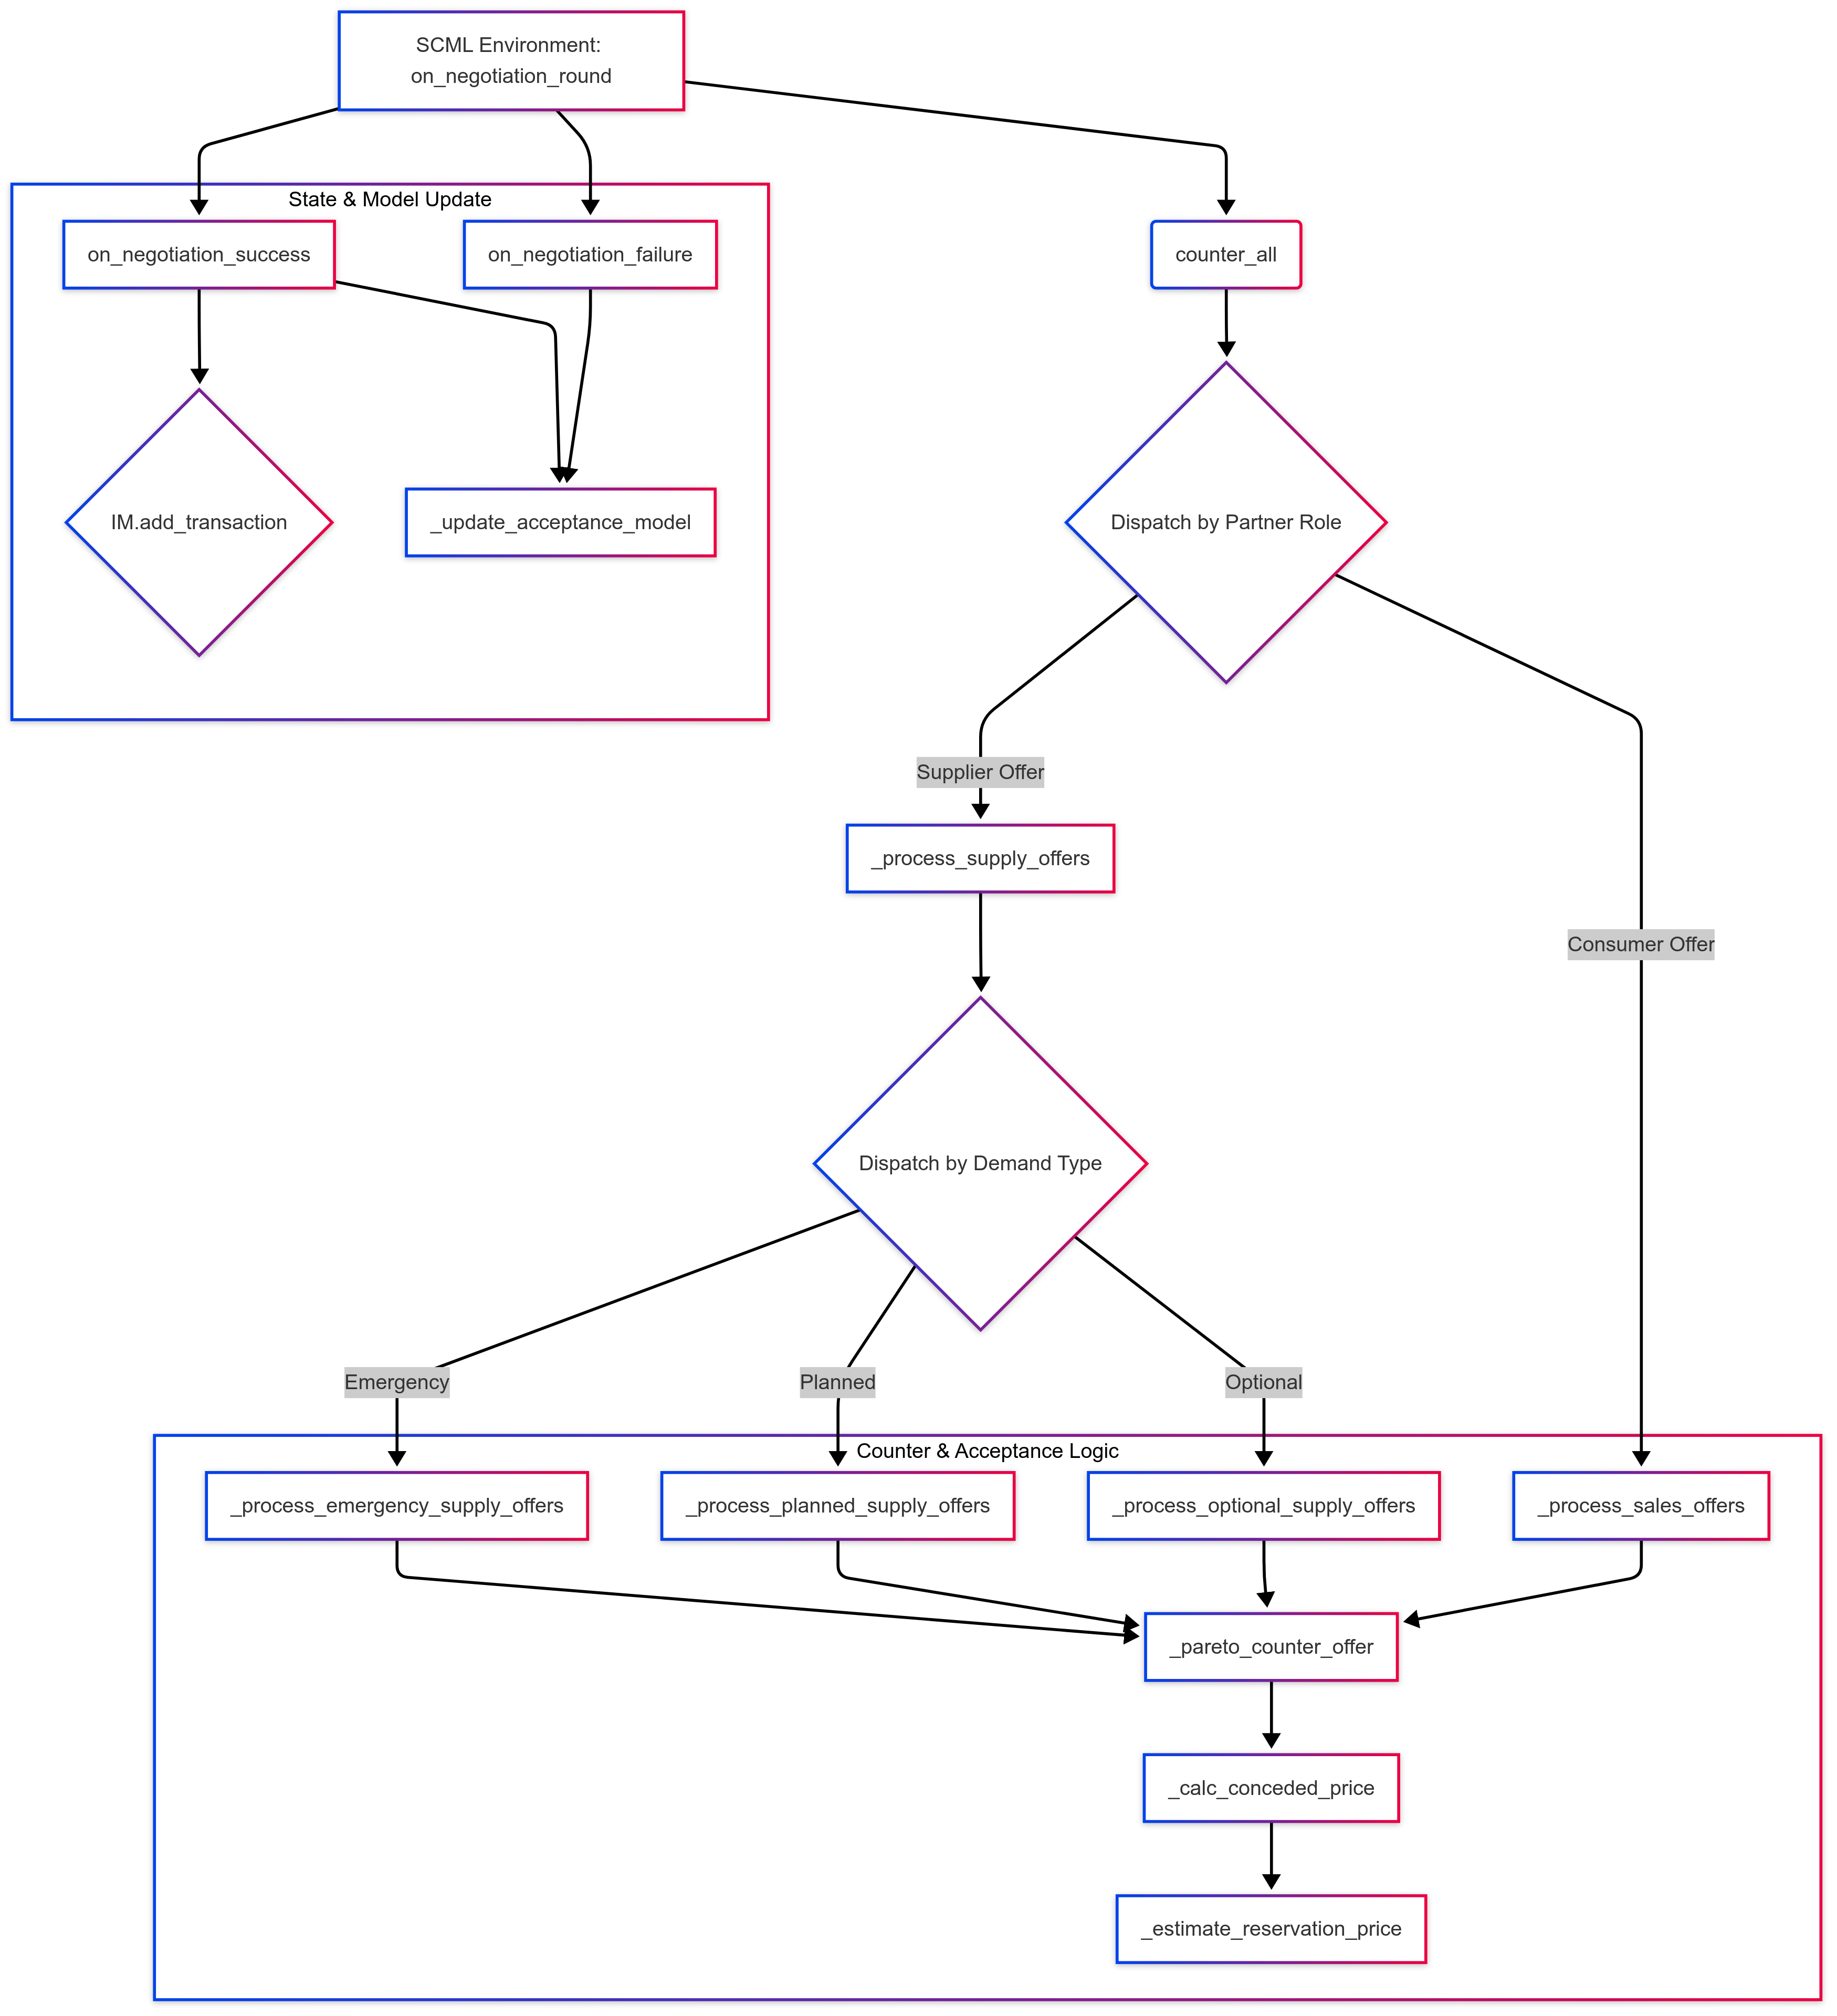
\includegraphics[width=0.5\linewidth]{Editor _ Mermaid Chart-2025-06-08-092514.png}
    \caption{Core Method Call Flow}
    \label{fig:enter-label}
\end{figure}
\section{Mathematical Formulation of Strategy}

\subsection{Acceptance Logic}
The agent's acceptance decisions are contextual and determined by the logical rules within four different processing modules.

\begin{enumerate}
\item \textbf{Emergency Supply}: An offer $(q_i, t_i, p_i)$ from supplier $i$ is accepted if $t_i$ is the current day and:
$$
\text{Accept if } (p_i \le \pi) \lor (p_i \le 1.1 \cdot \pi \land t_{\text{rel}} > 0.8)
$$
where $\pi$ is the \textbf{shortfall\_penalty} and $t_{\text{rel}}$ is the relative negotiation time.

\item \textbf{Planned Supply}: Acceptance requires satisfying both profitability and inventory capacity constraints.
\begin{itemize}
    \item \textbf{Profitability}: $p_{\text{eff}} \le p_{\text{max\_affordable}}$ \\
    where the effective price $p_{\text{eff}} = p_i + C_{\text{storage}} \cdot (t_i - t_{\text{today}} - 1)$ includes estimated storage costs. The maximum affordable price $p_{\text{max\_affordable}}$ is determined by the estimated future product selling price $\hat{S}$, processing cost $C_{\text{proc}}$, and minimum profit margin $m$:
    $$
    p_{\text{max\_affordable}} = \hat{S} \cdot (1 - m) - C_{\text{proc}}
    $$
    \item \textbf{Inventory Capacity}: $q_i \le H(t_i)$, where $H(t_i)$ is the procurement headroom at time $t_i$.
\end{itemize}

\item \textbf{Optional Supply}: 
$$
\text{Accept if } p_i \le \bar{p}_{\text{market}} \cdot \delta_{\text{bargain}} \land q_i \le H_{\text{opt}}(t_i)
$$
where $\bar{p}_{\text{market}}$ is the average market price and $\delta_{\text{bargain}}$ is the `bargain\_threshold`.

\item \textbf{Sales}:
$$
\text{Accept if } q_i \le C_{\text{avail}}(t_i) \land p_i \ge p_{\text{min\_sell}}
$$
where $C_{\text{avail}}(t_i)$ is the available production capacity at time $t_i$, and the minimum selling price $p_{\text{min\_sell}}$ is determined by costs and a dynamic profit margin $m_{\text{dynamic}}$:
$$
p_{\text{min\_sell}} = (C_{\text{raw\_avg}} + C_{\text{proc}}) \cdot (1 + m_{\text{dynamic}})
$$
\end{enumerate}

\subsection{Concession Logic}
The concession logic, implemented in \_calc\_conceded\_price, calculates a new counter-offer price $p^{\text{new}}$ in three steps.

\begin{enumerate}
\item \textbf{Concession Multiplier ($\beta$)}:
$$
\beta(t_{\text{rel}}, r_{\text{opp}}) = \min\left(1, t_{\text{rel}}^{\gamma} \cdot (1 + r_{\text{opp}})\right)
$$
where $t_{\text{rel}}$ is relative time, $r_{\text{opp}}$ is the opponent's relative concession rate, and $\gamma$ is the\textbf{ concession\_curve\_power}.

\item \textbf{Target Price Blending ($p^{\star}$)}: 
$$
p^{\star} = \frac{p_{\text{agent\_target}} + \hat{p}_{\text{opp}}}{2}
$$
where $p_{\text{agent\_target}}$ is the agent's ideal price for the round, and $\hat{p}_{\text{opp}}$ is the opponent's estimated reservation price from the opponent model.

\item \textbf{Final Price Calculation ($p^{\text{new}}$)}:
$$
p^{\text{new}} = p_0 + \beta \cdot (p^{\star} - p_0)
$$
where $p_0$ is the agent's initial anchor price (NMI max for sellers, NMI min for buyers).
\end{enumerate}

\subsection{Opponent Modeling}
The agent maintains an online logistic regression model for each partner to predict their acceptance probability and infer their reservation price.

\begin{enumerate}
\item \textbf{Model Definition}: The acceptance probability $P_{\text{acc}}$ is modeled as a Sigmoid function of price $p$:
$$
P_{\text{acc}}(p) = \sigma(w_0 + w_1 \cdot x) = \frac{1}{1 + e^{-(w_0 + w_1 \cdot x)}}
$$
The feature $x$ is defined as $x = p$ (for buying) or $x = -p$ (for selling).

\item \textbf{Model Update \textbf{(\_update\_acceptance\_model)}}: After each interaction, the weights $w_0, w_1$ are updated via stochastic gradient descent. With true label $y \in \{0, 1\}$ and prediction $\hat{y} = P_{\text{acc}}(p)$, the update rules are:
$$
\begin{align*}
w_0 & \leftarrow w_0 + \eta \cdot (y - \hat{y}) \\
w_1 & \leftarrow w_1 + \eta \cdot (y - \hat{y}) \cdot x
\end{align*}
$$
where $\eta$ is the learning rate \textbf{h.logreg\_learning\_rate}.

\item \textbf{Reservation Price Estimation (\textbf{\_estimate\_reservation\_price})}: The agent assumes the opponent's reservation price is where the acceptance probability is 50\%, which implies $w_0 + w_1 \cdot x_r = 0$. This gives the reservation feature value $x_r = -w_0 / w_1$, which is then converted back to a price $\hat{p}_{\text{opp}}$. This estimate is a key input for the concession logic's blended target price.
\end{enumerate}

\end{document}